% Capitolo 5 generato dalla bozza Markdown verificata.
\chapter{Domain-Specific Language e motore di verifica}\label{domain-specific-language-e-motore-di-verifica}

\section{Struttura della grammatica}\label{struttura-della-grammatica}

La sintassi del DSL è definita mediante una grammatica realizzata con Lark, una libreria Python per la costruzione di parser a partire da grammatiche formali. Le regole del linguaggio utilizzano i tipi semantici degli eventi e i relativi attributi, resi disponibili dalle fasi di normalizzazione e risoluzione semantica.

Una specifica è composta da istruzioni dedicate alla selezione delle evidenze e alla definizione dei criteri di verifica. La selezione può essere espressa attraverso \texttt{SEQUENCE}, che descrive una successione ordinata di eventi, oppure \texttt{COLLECT}, che raccoglie le occorrenze di un determinato tipo di evento. In entrambi i casi, la parola chiave \texttt{AS} permette di associare un identificatore simbolico, denominato alias, all'evidenza individuata. All'interno di \texttt{SEQUENCE} è inoltre possibile utilizzare \texttt{OPTIONAL} per indicare porzioni della sequenza la cui presenza non è obbligatoria.

I criteri di verifica sono definiti mediante \texttt{REQUIRE}, che consente di esprimere confronti tra valori letterali e campi degli eventi selezionati. Il linguaggio prevede inoltre \texttt{REQUIRE UNIQUE} per verificare proprietà di unicità e \texttt{IF} per applicare determinate regole soltanto quando una condizione è soddisfatta. Le proprietà temporali sono invece espresse mediante MFOTL.

\Needspace{19\baselineskip}
Le principali produzioni della grammatica sono riportate di seguito.

\par\noindent\begin{minipage}{\linewidth}
\begin{lstlisting}
start: statement+

?statement: sequence_rule
          | collect_rule
          | rule

?rule: static_rule
     | temporal_rule

?static_rule: comparison_rule
            | unique_rule
            | if_rule

sequence_rule: "SEQUENCE" "{" sequence_element+ "}"
?sequence_element: sequence_item | optional_block
sequence_item: FIELD "AS" NAME
optional_block: "OPTIONAL" "{" sequence_element+ "}"

collect_rule: "COLLECT" FIELD "AS" NAME

comparison_rule: "REQUIRE" FIELD OP operand
unique_rule: "REQUIRE" "UNIQUE" FIELD
if_rule: "IF" FIELD OP operand "{" rule+ "}"

temporal_rule: "MFOTL" "CASE" VALUE MFOTL_BLOCK

?operand: FIELD -> field_operand
        | VALUE -> literal_operand
\end{lstlisting}
\end{minipage}\par

I riferimenti agli eventi e ai relativi attributi sono rappresentati attraverso \texttt{FIELD}, che utilizza una notazione gerarchica separata da punti. Nella parte dedicata alla selezione, ad esempio, è possibile dichiarare:

\par\noindent\begin{minipage}{\linewidth}
\begin{lstlisting}
SEQUENCE {
    ausf.authentication.response AS initial_vector
    nas.authentication_request AS auth_request
}
\end{lstlisting}
\end{minipage}\par

In questo esempio, i due eventi semantici vengono associati rispettivamente agli alias \texttt{initial\_vector} e \texttt{auth\_request}, attraverso i quali è possibile accedere ai relativi campi nelle successive regole di verifica:

\par\noindent\begin{minipage}{\linewidth}
\begin{lstlisting}
REQUIRE auth_request.rand == initial_vector.rand
\end{lstlisting}
\end{minipage}\par

\texttt{NAME} identifica gli alias introdotti dalla specifica, mentre \texttt{VALUE} rappresenta valori letterali utilizzabili nelle espressioni. 



\section{Rappresentazione interna delle regole}\label{rappresentazione-interna-delle-regole}

Le istruzioni scritte nel DSL devono essere interpretate dal sistema per poter essere utilizzate durante la selezione e la verifica delle evidenze. A questo scopo, il parser costruito con Lark analizza la specifica e ne riconosce le strutture sintattiche, che vengono successivamente trasformate in rappresentazioni interne attraverso un \texttt{Transformer}.

Il matcher e i verificatori non operano quindi direttamente sul testo della DSL, ma su rappresentazioni strutturate che conservano esclusivamente le informazioni necessarie all'elaborazione.

A seconda dello statement considerato, vengono mantenute informazioni differenti, quali il tipo di operatore, i riferimenti ai campi, gli alias, gli operandi di confronto, eventuali regole annidate e, nel caso di proprietà temporali, la relativa formula.

Ad esempio, una regola come

\par\noindent\begin{minipage}{\linewidth}
\begin{lstlisting}
REQUIRE auth_request.rand == initial_vector.rand
\end{lstlisting}
\end{minipage}\par

viene trasformata concettualmente in una struttura del tipo:

\par\noindent\begin{minipage}{\linewidth}
\begin{lstlisting}
field: auth_request.rand
operator: ==
expected:
    type: field
    value: initial_vector.rand
\end{lstlisting}
\end{minipage}\par

In questo modo viene mantenuta anche la distinzione tra un operando costituito da un valore letterale e un operando che rappresenta invece il riferimento a un altro campo della specifica.

Per il costrutto \texttt{SEQUENCE}, la rappresentazione ottenuta dal parsing viene ulteriormente trasformata in un \emph{Abstract Syntax Tree} (AST) dedicato alla descrizione del pattern sequenziale. I tipi di nodo attualmente necessari sono:

\begin{itemize}
\tightlist
\item
  \texttt{Sequence}, che rappresenta l'insieme ordinato degli elementi del pattern;
\item
  \texttt{Atom}, associato a un singolo tipo di evento atteso e al relativo alias;
\item
  \texttt{Optional}, utilizzato per racchiudere elementi la cui presenza è opzionale.
\end{itemize}

Ad esempio, la specifica

\par\noindent\begin{minipage}{\linewidth}
\begin{lstlisting}
SEQUENCE {
    event.a AS a
    OPTIONAL {
        event.b AS b
    }
    event.c AS c
}
\end{lstlisting}
\end{minipage}\par

può essere rappresentata concettualmente attraverso il seguente albero:

\begin{verbatim}
Sequence
├── Atom(event.a, a)
├── Optional
│   └── Atom(event.b, b)
└── Atom(event.c, c)
\end{verbatim}


È importante precisare che non tutti gli elementi della DSL vengono trasformati nello stesso AST. La struttura composta da \texttt{Sequence}, \texttt{Atom} e \texttt{Optional} è specificamente utilizzata per rappresentare i pattern sequenziali, mentre le regole statiche e temporali vengono mantenute in strutture interne adatte ai rispettivi meccanismi di verifica.

Le rappresentazioni ottenute costituiscono quindi il livello di collegamento tra il parsing della specifica e i componenti incaricati della sua elaborazione.

Prima di procedere alla selezione dell'evidenza, viene inoltre effettuata una validazione strutturale degli alias utilizzati nei criteri statici. Questo controllo è necessario per verificare la coerenza dei riferimenti presenti nella specifica DSL, evitando che un alias utilizzato nelle regole di verifica, ma mai dichiarato, venga erroneamente interpretato come un'evidenza mancante durante l'analisi della cattura.

La validazione viene effettuata raccogliendo tutti gli alias dichiarati nella fase di selezione, a cui vengono aggiunti gli eventuali alias esterni, di configurazione o derivati. Questi vengono confrontati con gli alias utilizzati nelle regole di verifica, comprese le condizioni e le regole annidate. 

La validazione permette quindi di individuare gli alias utilizzati senza essere stati dichiarati, distinguendo gli errori presenti nella specifica dai casi in cui un alias correttamente dichiarato non risulti associato ad alcuna evidenza durante la selezione.


\section{Selezione mediante SEQUENCE}\label{selezione-mediante-sequence}

Questa sezione descrive il meccanismo utilizzato per individuare, all'interno del traffico osservato, le sequenze di eventi.

\subsection{Dal pattern all'automa}\label{il-pattern-sequenziale}

Per il riconoscimento dei pattern sequenziali, il sistema utilizza un automa a stati finiti non deterministico (\emph{Nondeterministic Finite Automaton}, NFA). Il pattern, precedentemente rappresentato mediante un AST, viene trasformato in un NFA che descrive i possibili percorsi di riconoscimento degli eventi.

Questa scelta permette di utilizzare un unico meccanismo di ricerca per sequenze con strutture differenti, comprese quelle contenenti blocchi \texttt{OPTIONAL}, senza dover sviluppare una logica di riconoscimento specifica per ciascun pattern.

\subsection{Formalizzazione dell'automa}\label{formalizzazione-dellautoma}

Formalmente, l'NFA adottato è definito dalla seguente quintupla:
\[
A = \langle \Sigma, \ Q, \ q_{0}, \ Q_{F}, \ \delta \rangle
\] dove

\begin{itemize}
\tightlist
\item
  \(\Sigma\) è l'alfabeto, costituito dall'insieme dei tipi semantici di evento riconosciuti dall'automa;
\item
  \(Q\) è l'insieme finito degli stati;
\item
  \(q_{0} \in Q\) è lo stato iniziale;
\item
  \(Q_{F} \subseteq Q\) è l'insieme degli stati finali. Nell'implementazione proposta viene utilizzato un unico stato di accettazione, pertanto \(Q_{F} = \{ q_{f} \}\);
\item
  \(\delta\) è la funzione di transizione non deterministica, definita come \[\delta: Q \times (\Sigma \ \cup \ \{  \varepsilon \}) \to \mathcal{P}(Q)\]
\end{itemize}

dove \(\mathcal{P}(Q) = 2^{Q}\) indica l'insieme delle parti di \(Q\), ossia l'insieme di tutti i suoi sottoinsiemi.



\subsection{\texorpdfstring{Le \(\varepsilon\)-transizioni}{Le \textbackslash varepsilon-transizioni}}\label{le-varepsilon-transizioni}

Una transizione ordinaria, etichettata con un simbolo \(a \in \Sigma\), può essere attraversata soltanto quando l'evento corrente della traccia presenta il tipo semantico richiesto. Il suo attraversamento comporta il consumo dell'evento e l'avanzamento nella lettura della traccia. Tale transizione è rappresentata come:

\[
q_{i} \xrightarrow{a} q_{j}
\]

Una transizione \(\varepsilon\), invece, ha la forma:

\[
q_{i} \xrightarrow{\varepsilon} q_{j}
\] e permette di passare da uno stato all'altro senza consumare alcun evento, ossia senza avanzare nella lettura della traccia.

Le \(\varepsilon\)-transizioni permettono quindi di collegare stati e percorsi dell'automa senza richiedere il riconoscimento di nuovi eventi. Questa caratteristica viene utilizzata nella costruzione di Thompson per combinare i diversi frammenti che compongono il pattern. 

\subsection{Compilazione del pattern mediante Thompson}\label{compilazione-del-pattern-mediante-thompson}

Una volta ottenuto l'AST, il pattern sequenziale viene compilato in un NFA mediante la costruzione di Thompson \cite{thompson_1968}. Tale procedimento si basa su un approccio composizionale: a ciascun nodo dell'albero viene associato un frammento dell'automa, dotato di uno stato iniziale e uno finale; i frammenti vengono successivamente collegati per ottenere l'automa corrispondente alla sequenza completa.

La costruzione dipende dal tipo di nodo considerato:

\begin{itemize}
\tightlist
\item
  \texttt{Atom}: genera un frammento costituito da due stati collegati da una transizione etichettata con il tipo semantico dell'evento atteso.
\item
  \texttt{Sequence}: combina i frammenti dei propri elementi nell'ordine specificato, collegando lo stato finale di ciascun frammento allo stato iniziale del successivo mediante una transizione \(\varepsilon\).
\item
  \texttt{Optional}: il blocco viene rappresentato mediante due percorsi alternativi collegati da transizioni \(\varepsilon\): uno attraversa il frammento corrispondente agli eventi opzionali, mentre l'altro consente di saltarlo senza consumare tali eventi.
\end{itemize}

Considerando il pattern sequenziale già introdotto nella Sezione~\ref{rappresentazione-interna-delle-regole}, la Figura~\ref{fig:thompson} ne mostra una rappresentazione schematica mediante NFA, ottenuta applicando la costruzione di Thompson ai nodi dell'AST.

\begin{figure}[H]
    \centering
    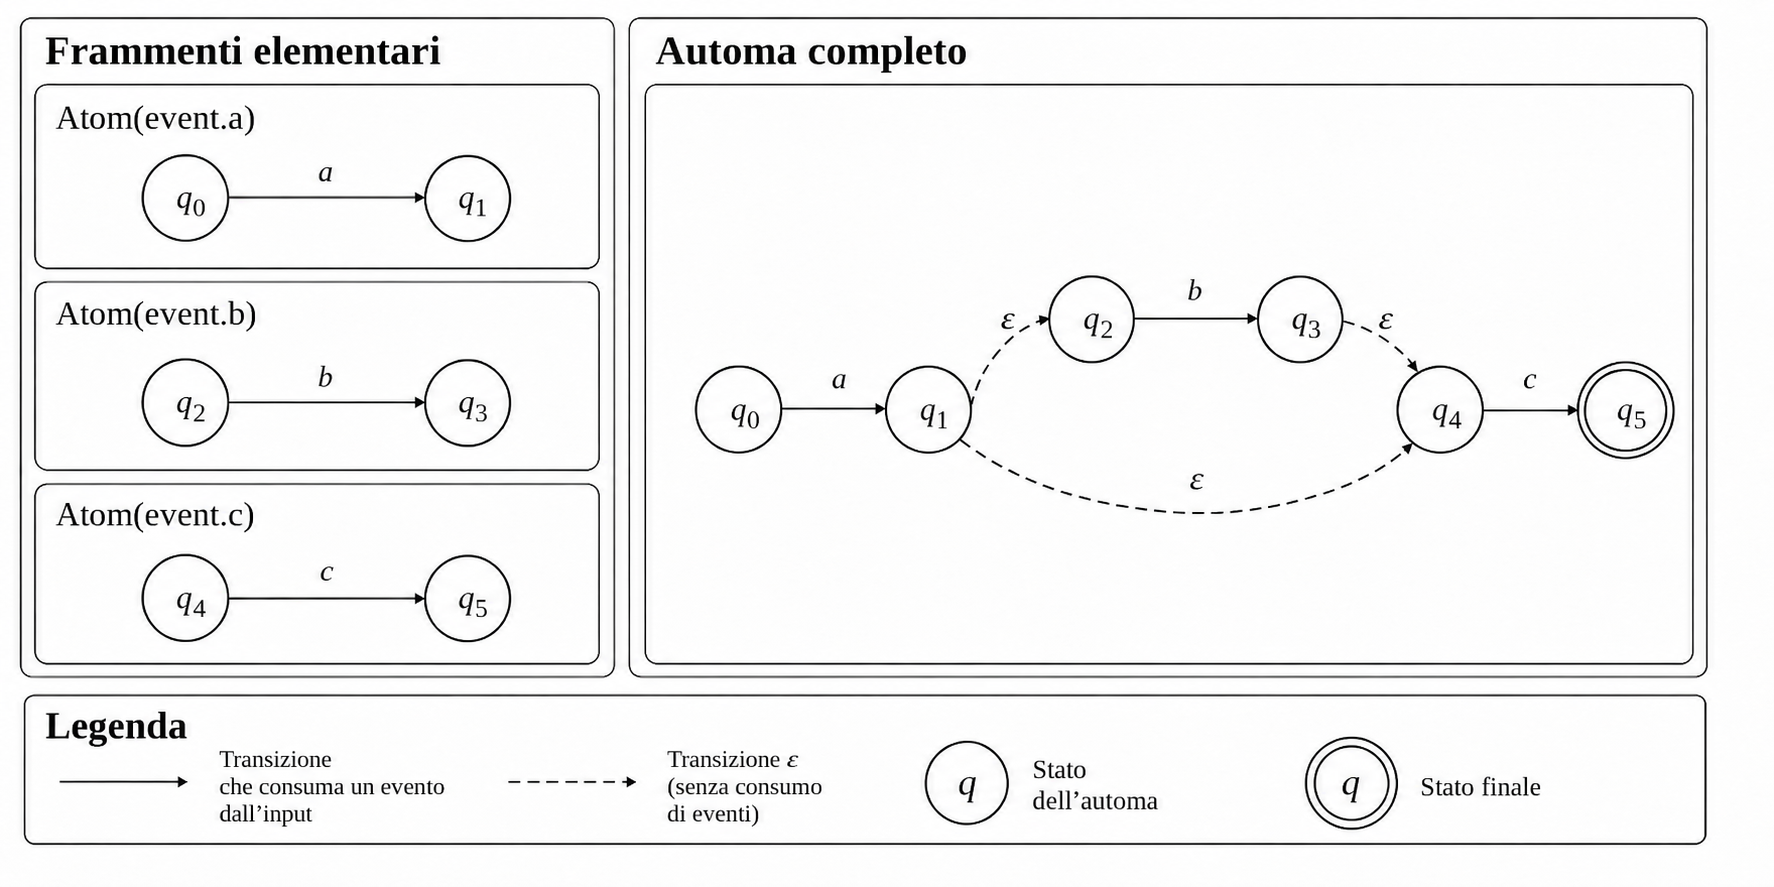
\includegraphics[
        width=\textwidth,
        height=0.65\textheight,
        keepaspectratio
    ]{figure/nfa_thompson.png}
    \caption{Rappresentazione schematica semplificata di un NFA per una sequenza contenente un blocco opzionale.}
    \label{fig:thompson}
\end{figure}

\subsection{Funzionamento del matcher}\label{configurazioni-attive-e-riconoscimento-degli-eventi}

Il riconoscimento delle sequenze di eventi all'interno della traccia è affidato al matcher, il componente che utilizza l'NFA per individuare le corrispondenze con il pattern definito nella DSL. Il matcher riceve in ingresso l'automa e la sequenza ordinata di \texttt{MessageEvent}, esaminando gli eventi per individuare i percorsi che consentono di raggiungere uno stato accettante.

Durante questa operazione non è sufficiente conoscere lo stato raggiunto nell'automa, poiché è necessario conservare anche i riferimenti agli eventi che hanno contribuito al riconoscimento. A questo scopo viene introdotta una struttura denominata \texttt{ActiveConfiguration}, formalizzabile come:

\[
C = \langle q, B \rangle
\]

dove

\begin{itemize}
\tightlist
\item
  \(q \in Q\) è lo stato corrente dell'automa;
\item
  \(B\) è una funzione parziale che associa gli alias definiti nella DSL ai \texttt{MessageEvent} già riconosciuti.
\end{itemize}

Il matcher può mantenere contemporaneamente più configurazioni attive, ciascuna caratterizzata dal proprio stato e dai binding progressivamente costruiti.

Poiché l'automa può contenere transizioni \(\varepsilon\), per ogni stato corrente devono essere considerati anche quelli raggiungibili senza consumare ulteriori eventi. A tale scopo viene utilizzata una \(\varepsilon \text{-closure}\), definita formalmente come:

\[
\varepsilon\text{-closure}(q) = \{ p \in Q \mid q \xrightarrow{ \ \ \varepsilon^{*} \ } p\}
\]

La chiusura comprende tutti gli stati raggiungibili da \(q\) attraverso zero o più transizioni \(\varepsilon\), incluso lo stesso \(q\). L'espansione di una configurazione attraverso tali transizioni mantiene invariati i binding già acquisiti, poiché non viene riconosciuto alcun nuovo evento.

Durante la scansione della traccia, il matcher confronta il \texttt{message\_type} di ciascun evento con quello richiesto dalle transizioni uscenti dagli stati delle configurazioni attive. Quando viene individuata una transizione compatibile, la configurazione avanza verso lo stato di destinazione e il \texttt{MessageEvent} osservato viene associato all'alias definito nel corrispondente \texttt{Atom}. I binding vengono quindi aggiornati e vengono considerate le ulteriori transizioni \(\varepsilon\) raggiungibili dal nuovo stato.

Una caratteristica importante è che la selezione non richiede che gli eventi previsti dal pattern siano consecutivi nella traccia. Quando un evento non può essere consumato da una determinata configurazione, quest'ultima può rimanere attiva, consentendo di proseguire la ricerca con gli eventi successivi.

La possibilità di mantenere più configurazioni attive consente inoltre al matcher di seguire simultaneamente le alternative previste dall'NFA in presenza di blocchi \texttt{OPTIONAL}, comprese le configurazioni raggiungibili mediante \(\varepsilon\)-transizioni che consentono di omettere gli eventi opzionali.

\subsection{Avvio e riavvio dei candidati}\label{politica-di-matching-e-produzione-dei-risultati}

All'interno di una cattura possono essere presenti più occorrenze degli eventi descritti dalla stessa \texttt{SEQUENCE}, anche in posizioni differenti della traccia. Il matcher esamina quindi gli eventi in ordine e, per ogni posizione compatibile con l'inizio del pattern, avvia un nuovo candidato di riconoscimento. Ciascun candidato rappresenta un tentativo indipendente di completare la sequenza a partire dalla posizione individuata e può mantenere più configurazioni attive, corrispondenti ai diversi percorsi dell'automa.

Durante l'elaborazione viene applicata una politica di riavvio (\emph{restart policy}), finalizzata a evitare che eventi appartenenti a tentativi distinti vengano associati alla stessa sequenza. Se viene incontrato un evento compatibile con l'inizio di un nuovo candidato, ma che non può essere consumato da nessuna delle configurazioni attive del candidato corrente, quest'ultimo viene interrotto. L'evento potrà comunque essere considerato come punto di partenza di un candidato distinto.

\subsection{Produzione e filtraggio dei match}\label{produzione-e-filtraggio-dei-match}

Un candidato completa il riconoscimento quando almeno una delle sue configurazioni raggiunge lo stato accettante dell'NFA. Per ciascun candidato viene considerato il primo punto di completamento, nel quale possono tuttavia essere presenti più configurazioni accettanti, associate a percorsi differenti dell'automa.

A ogni configurazione accettante corrisponde un oggetto \texttt{Match}, che conserva la posizione iniziale del candidato (\texttt{start\_index}), quella in cui è stato completato il riconoscimento (\texttt{end\_index}) e i binding degli eventi individuati. Il matcher può quindi produrre più match, anche a partire da uno stesso candidato.

La presenza di percorsi alternativi, in particolare quelli introdotti da \texttt{OPTIONAL}, può produrre match riferiti allo stesso intervallo della traccia ma contenenti binding differenti. Per eliminare i risultati meno completi senza perdere evidenze distinte, viene applicato un criterio di dominanza: un match domina un altro quando sono soddisfatte tutte le seguenti condizioni.

\begin{itemize}
\tightlist
\item
  i due match condividono \texttt{start\_index} e \texttt{end\_index};
\item
  gli alias del secondo costituiscono un sottoinsieme proprio di quelli del primo;
\item
  per tutti gli alias comuni, le associazioni fanno riferimento agli stessi eventi osservati.
\end{itemize}

Il filtraggio elimina quindi soltanto i match dominati, conservando quelli che presentano associazioni differenti o che non sono confrontabili secondo tali condizioni.

Al termine del filtraggio, il matcher restituisce i match completi non dominati, che costituiscono il risultato della selezione sequenziale e contengono le associazioni tra gli alias e gli eventi riconosciuti.

\section{Selezione mediante COLLECT}\label{selezione-mediante-collect}

La selezione mediante \texttt{COLLECT} viene effettuata confrontando il tipo semantico dichiarato nella regola con il campo \texttt{message\_type} degli eventi disponibili. Tutte le occorrenze corrispondenti vengono raccolte e associate all'alias specificato, senza richiedere la costruzione di un automa.

Una regola di raccolta può essere espressa come segue:

\par\noindent\begin{minipage}{\linewidth}
\begin{lstlisting}
COLLECT pfcp.session_establishment_response AS responses
\end{lstlisting}
\end{minipage}\par

In questo esempio, \texttt{pfcp.session\_establishment\_response} identifica il tipo di evento da ricercare, mentre \texttt{responses} è l'alias assegnato alla collezione risultante.

Gli eventi individuati vengono associati all'alias all'interno del \texttt{BindingContext}. A differenza di \texttt{SEQUENCE}, dove ciascun alias identifica un singolo evento riconosciuto, nel caso di \texttt{COLLECT} il valore associato è una lista di \texttt{MessageEvent}, rappresentabile come:

\[
B(\texttt{responses}) = [e_1, e_2, e_3, ..., e_n]
\] La struttura del \texttt{BindingContext} rimane quindi invariata, mentre cambia la natura dell'evidenza associata all'alias. Le due modalità di selezione, pur adottando meccanismi differenti, producono così una rappresentazione comune dei risultati.

\section{Verifica statica}\label{verifica-statica}

Il verificatore statico utilizza i binding presenti nel \texttt{BindingContext} per valutare i criteri definiti nelle regole DSL. Per effettuare le verifiche, riceve il contesto prodotto dalla selezione e le regole ottenute durante il parsing della specifica.

\Needspace{7\baselineskip}
Le regole di confronto sono introdotte dalla parola chiave \texttt{REQUIRE} e possono essere espresse nella forma generale:

\par\noindent\begin{minipage}{\linewidth}
\begin{lstlisting}
REQUIRE alias.campo OP valore
\end{lstlisting}
\end{minipage}\par

dove OP identifica l'operatore di confronto, mentre l'operando a destra può essere un valore letterale oppure un riferimento a un altro campo.

Per effettuare la valutazione, il verificatore deve innanzitutto risolvere i riferimenti presenti nella regola. Nel caso di un binding associato a un singolo evento, viene individuato l'alias interno del \texttt{BindingContext} e recuperato il relativo \texttt{MessageEvent}. Il percorso gerarchico specificato nella DSL viene quindi utilizzato per accedere ai campi, anche annidati, contenuti nell'attributo \texttt{fields} dell'evento. Quando invece il binding contiene una collezione, il campo richiesto viene recuperato da ciascuna evidenza, conservando anche il riferimento ai frame da cui proviene. Il medesimo meccanismo consente inoltre di accedere a informazioni esterne o derivate, eventualmente aggiunte al \texttt{BindingContext}, attraverso gli stessi riferimenti gerarchici utilizzati per gli eventi selezionati.

Una volta risolti i riferimenti presenti nella regola, il verificatore dispone dei valori necessari per applicare il criterio richiesto. La valutazione può consistere nel confronto tra due valori oppure nel controllo dell'unicità degli elementi di una collezione. In quest'ultimo caso, vengono considerate anche informazioni strutturate o contenenti più valori, conservando i riferimenti ai frame degli eventuali duplicati individuati.

La valutazione può inoltre dipendere da una condizione definita mediante \texttt{IF}. Quando la condizione è soddisfatta, il verificatore esegue le regole contenute nel blocco; in caso contrario, queste non vengono valutate e il blocco assume lo stato \texttt{SKIPPED}. Tale stato indica che le verifiche condizionali non sono applicabili e non rappresenta un ulteriore verdetto del test.

Ogni criterio valutato produce un risultato strutturato che associa l'esito alle informazioni utilizzate nella verifica, come i valori osservati e attesi e, quando pertinenti, i riferimenti ai frame. Questi risultati costituiscono la base per la successiva determinazione del verdetto complessivo.

\section{Verifica temporale}\label{verifica-temporale}

La verifica temporale permette di valutare proprietà che dipendono non soltanto dai valori contenuti nei messaggi, ma anche dalle relazioni temporali tra gli eventi osservati. A questo scopo viene utilizzata la \emph{Metric First-Order Temporal Logic} (MFOTL) \cite{basin_mfotl_2015}, un formalismo che consente di esprimere proprietà mediante predicati e operatori temporali, associando a questi ultimi intervalli entro cui devono essere soddisfatte determinate condizioni.

Le formule vengono valutate attraverso MonPoly \cite{basin_monpoly_2017}, un motore di monitoraggio esterno che verifica proprietà MFOTL su tracce temporizzate. La formula descrive quindi la proprietà richiesta, mentre MonPoly ne valuta il soddisfacimento rispetto agli eventi osservati.

\Needspace{10\baselineskip}
All'interno del DSL, una proprietà temporale può essere dichiarata mediante il costrutto \texttt{MFOTL CASE}. Il seguente esempio, tratto dal test AMF Synchronization Failure -- Case A, richiede che a una richiesta di risincronizzazione segua una risposta AUSF entro un intervallo temporale configurato.

\par\noindent\begin{minipage}{\linewidth}
\begin{lstlisting}
MFOTL CASE A """
ResynchronizationRequest()
IMPLIES
EVENTUALLY[0,{TIMER_MS}] AusfAuthenticationResponse()
"""
\end{lstlisting}
\end{minipage}\par

Per valutare la formula, MonPoly richiede una traccia temporizzata, nella quale gli eventi sono rappresentati mediante predicati associati ai rispettivi timestamp. Il sistema costruisce questa traccia a partire dagli eventi riconosciuti durante la selezione, utilizzando la configurazione del test per stabilire la corrispondenza tra gli alias della DSL e i predicati della formula.

La stessa configurazione indica il file di \emph{signature}, nel quale sono dichiarati i nomi dei predicati e gli eventuali argomenti che MonPoly può riconoscere. Nell'esempio precedente, tra i predicati utilizzati figurano \texttt{ResynchronizationRequest()} e \texttt{AusfAuthenticationResponse()}. Prima dell'esecuzione, il parametro \texttt{\{TIMER\_MS\}} viene sostituito con il valore configurato per il test, espresso in millisecondi.

Una volta preparate la formula, la signature e la traccia temporizzata, il sistema avvia MonPoly per effettuare la verifica. Nell'implementazione sviluppata viene utilizzata l'opzione \texttt{-negate}, che consente di monitorare la negazione della proprietà specificata e quindi di individuare le eventuali violazioni della formula originale. L'output prodotto da MonPoly viene infine interpretato dal verificatore per determinare l'esito del controllo temporale.

\section{Determinazione del verdetto}\label{determinazione-del-verdetto}

Il risultato della verifica di un caso di test è espresso attraverso uno dei tre verdetti previsti dal sistema: \texttt{PASS}, quando i criteri richiesti risultano soddisfatti; \texttt{FAIL}, quando viene rilevata una violazione; e \texttt{INCONCLUSIVE}, quando le evidenze disponibili non consentono di determinare un esito conclusivo.

Il verdetto \texttt{INCONCLUSIVE} viene prodotto quando le evidenze disponibili non consentono di valutare in modo conclusivo i criteri del caso di test. Questa situazione può verificarsi già durante la selezione: nel caso di \texttt{SEQUENCE}, quando non viene individuato alcun match completo oppure quando, anche dopo il filtraggio, rimangono più corrispondenze complete; nel caso di \texttt{COLLECT}, quando non sono presenti eventi del tipo semantico richiesto. L'impossibilità di concludere la verifica può emergere anche successivamente, qualora un criterio statico applicabile richieda un alias al quale non è stato associato alcun evento, come può accadere per un blocco \texttt{OPTIONAL} non attraversato durante il riconoscimento. In quest'ultimo caso, il verificatore non dispone dei valori necessari per valutare la regola: l'assenza dell'evidenza richiesta non permette di stabilire né il soddisfacimento né la violazione del criterio.

\Needspace{18\baselineskip}
Quando il caso di test prevede più criteri di verifica, i rispettivi risultati vengono combinati secondo una logica a tre valori, riportata nella Tabella~\ref{tab:aggregazione-tre-valori}.

\begin{center}
\begin{minipage}{0.88\textwidth}
\centering
\begingroup
\small
\renewcommand{\arraystretch}{1.18}
\begin{tabularx}{\linewidth}{|>{\centering\arraybackslash}X|>{\centering\arraybackslash}X|>{\centering\arraybackslash}X|}
\hline
\rowcolor{blue!7}
\textbf{Criterio A} & \textbf{Criterio B} & \textbf{Risultato} \\
\hline
PASS & PASS & PASS \\
\hline
PASS & FAIL & FAIL \\
\hline
PASS & INCONCLUSIVE & INCONCLUSIVE \\
\hline
FAIL & PASS & FAIL \\
\hline
FAIL & FAIL & FAIL \\
\hline
FAIL & INCONCLUSIVE & FAIL \\
\hline
INCONCLUSIVE & PASS & INCONCLUSIVE \\
\hline
INCONCLUSIVE & FAIL & FAIL \\
\hline
INCONCLUSIVE & INCONCLUSIVE & INCONCLUSIVE \\
\hline
\end{tabularx}
\endgroup
\captionof{table}{Tabella di aggregazione dei risultati di verifica secondo una logica a tre valori.}
\label{tab:aggregazione-tre-valori}
\end{minipage}
\end{center}

Come mostrato nella Tabella~\ref{tab:aggregazione-tre-valori}, il verdetto complessivo è \texttt{PASS} quando tutti i criteri applicabili risultano soddisfatti e \texttt{FAIL} quando almeno uno di essi rileva una violazione. \texttt{INCONCLUSIVE} viene invece prodotto quando non sono state rilevate violazioni, ma almeno un criterio non può essere valutato. Le regole contrassegnate come \texttt{SKIPPED} sono escluse dall'aggregazione, poiché non applicabili.

La stessa logica viene utilizzata quando il caso di test prevede sia verifiche statiche sia temporali, combinando i rispettivi risultati per determinare un unico verdetto complessivo.


